\documentclass[14pt]{beamer}
\usetheme{Frankfurt}
\usepackage[utf8]{inputenc}
\usepackage[russian]{babel}
\usepackage[OT1]{fontenc}
\usepackage{amsmath}
\usepackage{amsfonts}
\usepackage{amssymb}
\usepackage{graphicx}
\author{Гарифуллин Альберт}
\title{Approximate instancing method for plant ecosystems modeling}
%\setbeamercovered{transparent} 
%\setbeamertemplate{navigation symbols}{} 
%\logo{} 
\institute{Московский Государственный Университет\linebreak
		   факультет Вычислительной Математики и Кибернетики\linebreak
		   лаборатория Компьютерной графики и Мультимедиа} 
\date{28.09.21} 
%\subject{} 
\begin{document}

\begin{frame}
\titlepage
\end{frame}

%\begin{frame}
%\tableofcontents
%\end{frame}
  
\begin{frame}{Проблемы процедурной генерации}
 - Использовать много уникальных моделей напрямую не позволяют ограничения
   памяти\linebreak	
 - Использование небольшого числа заранее подготовленных моделей не обеспечивает желаемого разнообразия\linebreak	
 
 Как сохранить реалистичность и разнообразие процедурно генерируемых растений без необходимости хранить детализированные модели?
\end{frame}

\begin{frame}{General pipeline}
\begin{figure}[hbtp]
\includegraphics[scale=0.57]{pipeline.png}
\end{figure}
- Внешний генератор создает деревья в определенном формате\linebreak	
- Они трансформируются в компактное представление\linebreak	
- Результат может быть сконвертирован для хранения и использования - например, в GLTF-сцену\linebreak	
\end{frame}

\begin{frame}{Approximate instancing}
По множеству уникальных деревьев построить набор базовых структурных элементов, из которых, используя простые геометрические преобразования, можно получить деревья, внешне минимально отличающиеся от исходных.
\begin{figure}[hbtp]
\includegraphics[scale=0.25]{approximate_inst.png}
\end{figure}
\end{frame}

\begin{frame}{Кластеризация}
Дерево представляется как структура, состоящая из ствола и веток, растущих из него. \linebreak	
Множества все стволов и веток множества деревьев по отдельности проходят процедуру кластеризации - разделение на группы структурно похожих между собой элементов.\linebreak	
Все элементы одного кластера заменяются на instance типичного представителя\linebreak	
\end{frame}
\begin{frame}{Кластеризация}
\begin{figure}[hbtp]
\includegraphics[scale=0.56]{Clustering.png}
\end{figure}
\end{frame}
\begin{frame}{Функция дистанции}
 - Приведение веток в нормализованную форму\linebreak	
 - Сравнение вокселизированных моделей \linebreak	
 - Поиск структурных соответствий - попарное соотнесение узлов друг с другом

\end{frame}
\begin{frame}{Результат}
\begin{figure}[hbtp]
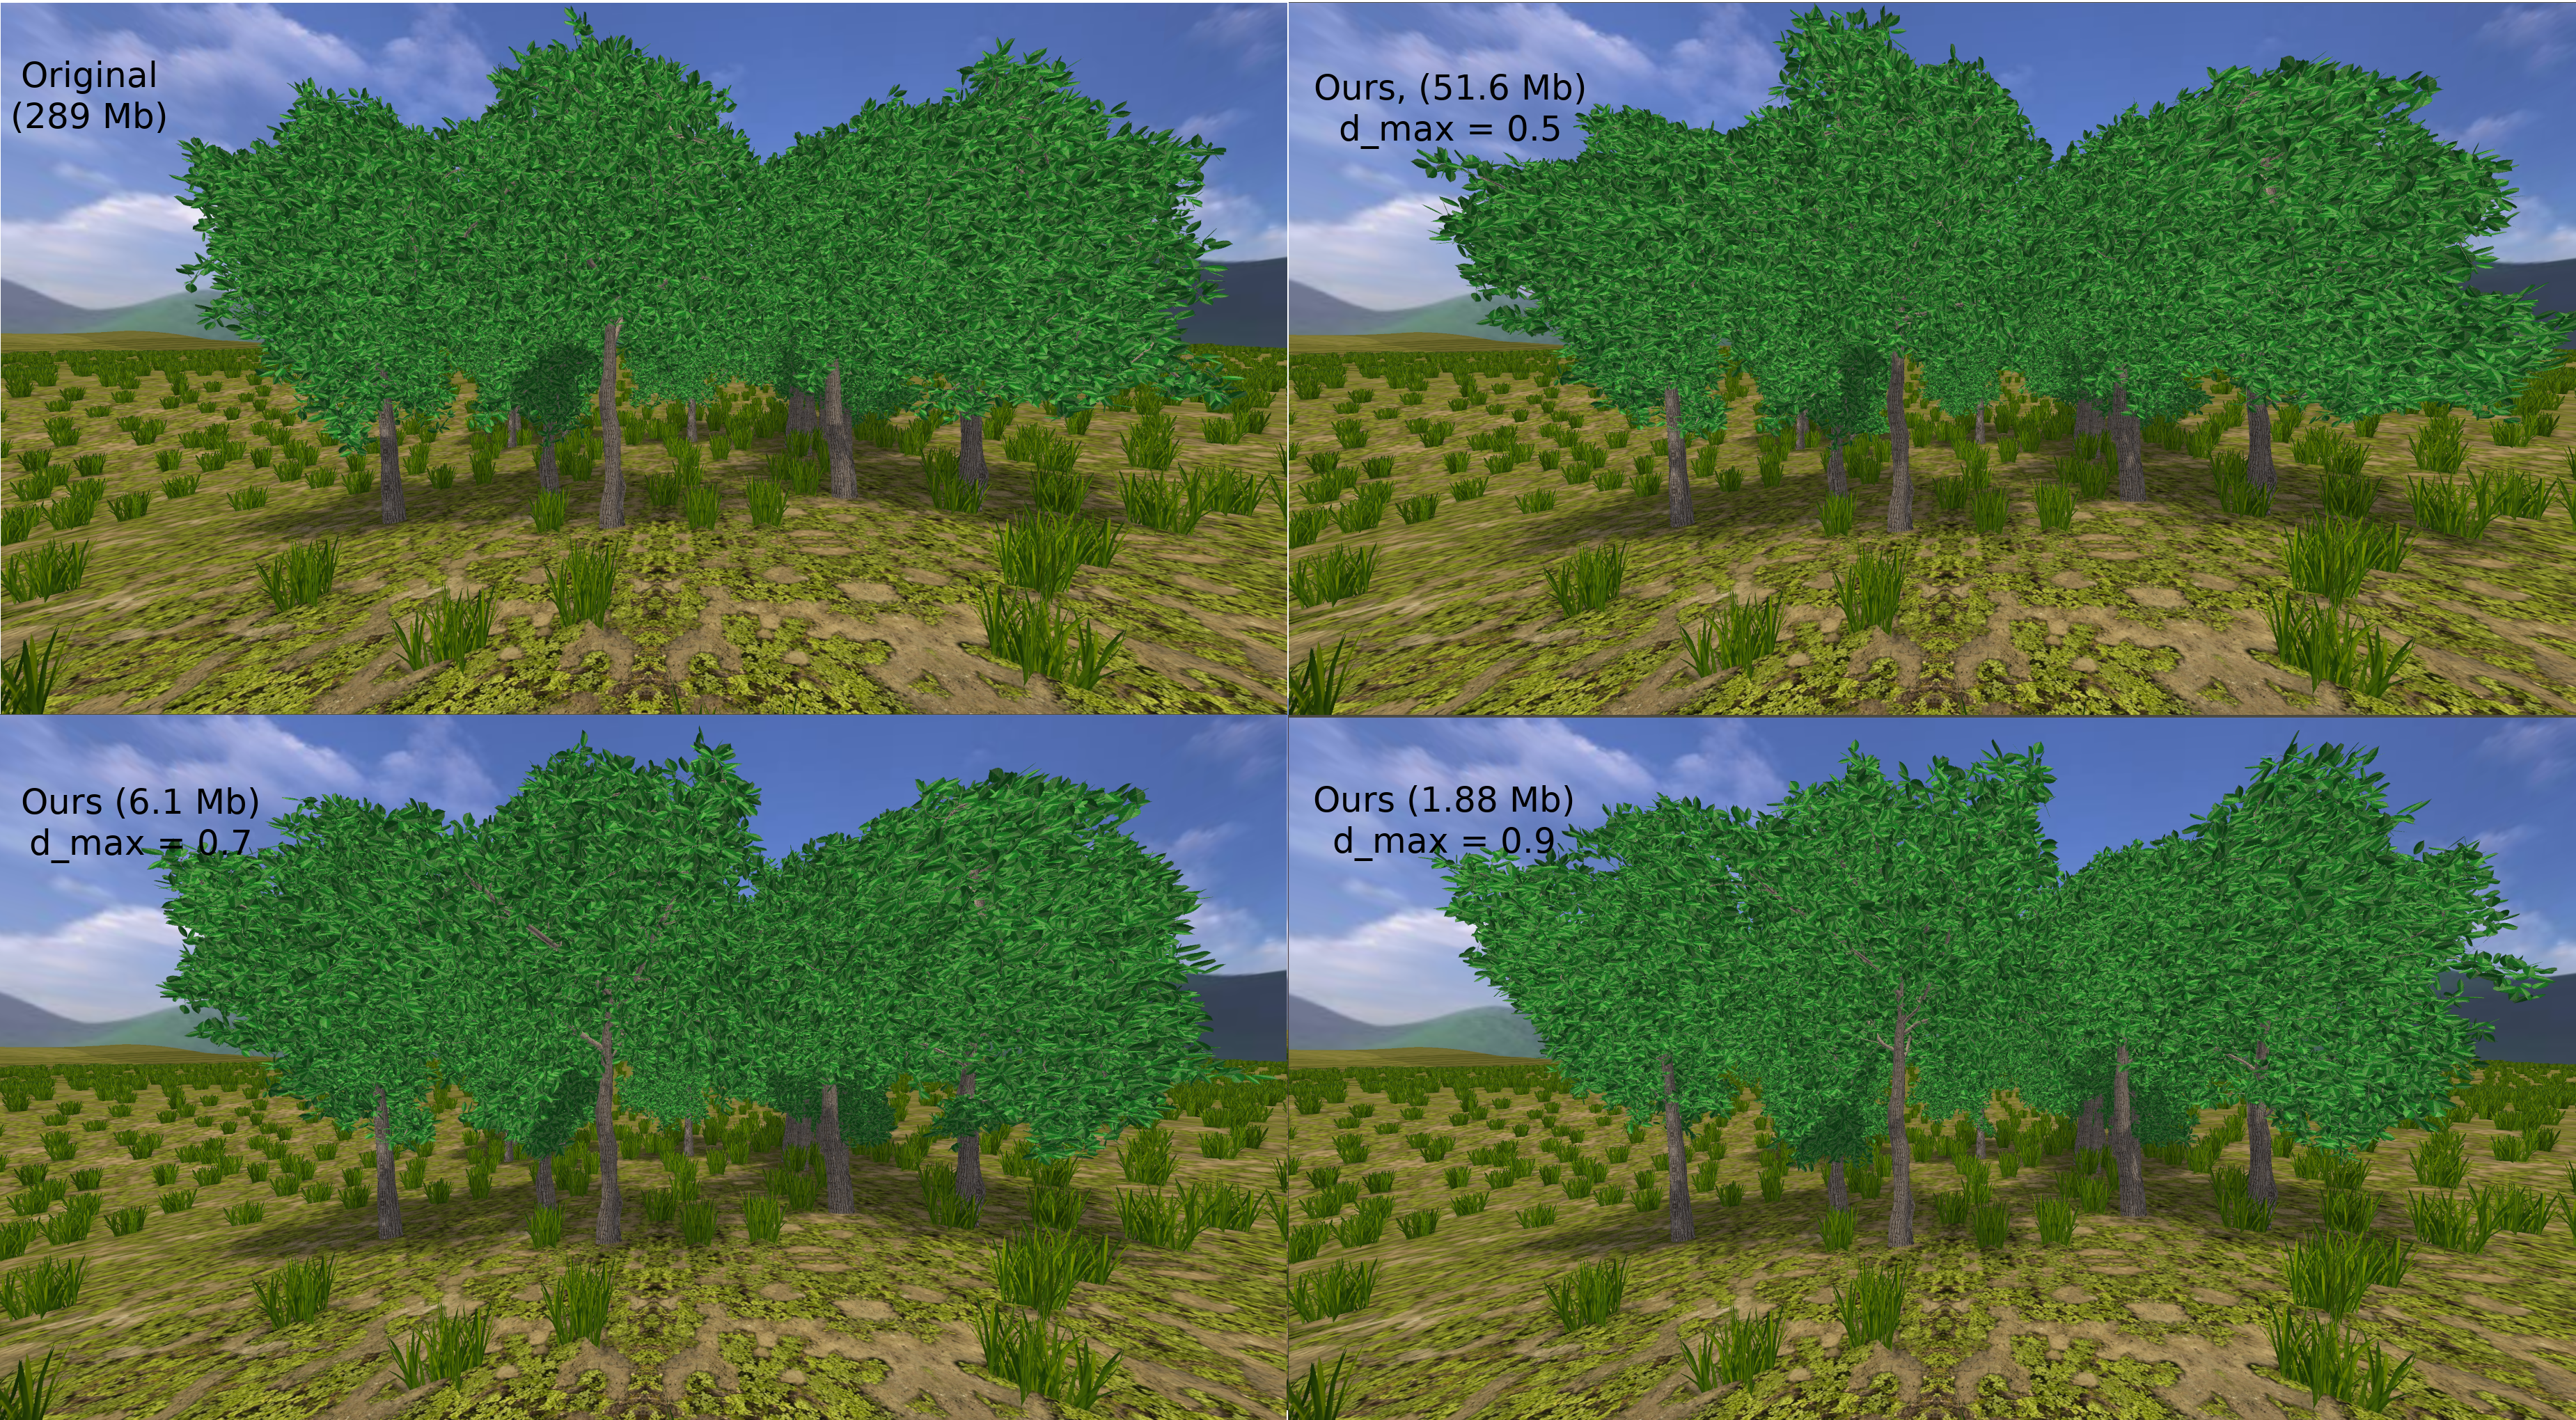
\includegraphics[scale=0.085]{comparison_1.png}
\end{figure}
\end{frame}
\begin{frame}{Результат}
\begin{figure}[hbtp]
\includegraphics[scale=0.15]{comparison_2.png}
\end{figure}
\end{frame}

\begin{frame}{Кластеризация}
MID - максимальная индивидуальная дистанция между элементами
кластера.
Эффективность повышается при увеличении числа объектов в исходной группе
\begin{figure}[hbtp]
\includegraphics[scale=0.58]{stat2.png}
\end{figure}
\end{frame}
\begin{frame}{Кластеризация}
\begin{figure}[hbtp]
\includegraphics[scale=0.6]{stat3.png}
\end{figure}
\end{frame}

\begin{frame}{"Синтетические деревья"}
 - Генератор может работать очень медленно\linebreak	
 - Деревья в больших группах могут быть менее реалистичны в деталях \linebreak	
 - Можно создавать новые деревья из уже имеющихся моделей

\end{frame}

\begin{frame}{"Синтетические деревья"}
\begin{figure}[hbtp]
\includegraphics[scale=0.57]{Synts.png}
\end{figure}
\end{frame}
\begin{frame}{Результат}	
\begin{figure}[hbtp]
\includegraphics[scale=0.18]{synt_comparison_1.png}
\end{figure}
\end{frame}
\begin{frame}{Преимущества}
1) Сохраняется уникальность деревьев\linebreak	
2) Алгоритм не зависит от процедур генерации\linebreak	
3) Результатом работы алгоритма являются структуры данных, типичные для описания растительности на сцене. Для их рендера можно использовать уже существующие алгоритмы.
\end{frame}

\begin{frame}{Конец}
Спасибо за внимание!
\end{frame}
\end{document}